\documentclass[../main/main.tex]{subfiles}

\raggedbottom

\makeatletter
\renewcommand{\@chapapp}{Optique -- chapitre}
\makeatother

\begin{document}
\setcounter{chapter}{2}

\chapter{Miroir plan et lentilles minces}

\section{Miroir plan}

\subsection{Définition}

\begin{tcbraster}[raster columns=2, raster equal height=rows]
    \begin{defi}[label=def:mir]{miroir plan}
        Surface plane totalement réfléchissante. On le schématisme avec le symbole
        \begin{center}
            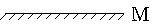
\includegraphics[width=4cm]{mir_plan.pdf}
        \end{center}
        pour un miroir orienté vers le haut.
    \end{defi}
    \begin{ror}[label=mirstig]{stigmatisme et aplanétisme des miroirs plans}
        Le miroir plan est le seul système optique rigoureusement stigmatique et
        aplanétique.
    \end{ror}
\end{tcbraster}

\subsection{Construction de l'image d'un objet réel}

On utilise les lois de Snell-Descartes pour la réflexion, en traçant deux rayons
partant de l'objet ponctuel.

\begin{exem}[label=exem:mir, sidebyside]{image d'un objet réel}
    Soit $A$ un point objet d'un miroir plan. Les rayons incidents se croisant
    en $A$ arrivent sur le miroir en $I$ et $I'$. Par la loi de la réflexion,
    les rayons émergents sont les rayons réfléchis, avec un angle de réflexion
    opposé à l'angle d'incidence. On trouve l'image $A'$ en traçant
    l'intersection des rayons émergents. \bigbreak
    Avec la figure ci-contre, on observe
    \[\tan(i) = \frac{\obar{HI}}{\obar{HA}} = \frac{\obar{HI}}{-\obar{HA'}}\]
    Soit \[ \boxed{\obar{HA'} = -\obar{HA}}\]
    \tcblower
    \begin{center}
        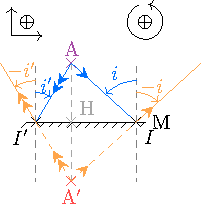
\includegraphics[width=\linewidth]{mir_plan-obj_r.pdf}
        \captionof{figure}{Construction de l'image d'un objet réel par un miroir
        plan.}
        \label{fig:mir_plan-obj_r}
    \end{center}
\end{exem}

\newpage

\subsection{Construction de l'image d'un objet virtuel}

\begin{exem}[label=exem:mir, sidebyside,
    righthand width=.2\linewidth]{image d'un objet réel}

    Le principe du retour inverse de la lumière permet de permuter $A$ et $A'$
    dans la démonstration précédente. Le schéma est cependant indiqué ci-contre
    (à compléter).

    \tcblower
    \begin{center}
        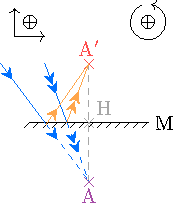
\includegraphics[width=\linewidth]{mir_plan-obj_v.pdf}
        \captionof{figure}{
            %Construction de l'image d'un objet virtuel par un miroir plan.
        }
        \label{fig:mir_plan-obj_v}
    \end{center}
\end{exem}

\subsection{Relation de conjugaison}

\begin{tcbraster}[raster columns=8, raster equal height=rows]
    
    \begin{defi}[label=def:relconj, raster multicolumn=2, heart]{Relation de
        conjugaison}

        Formule mathématique reliant la position d'un objet à celle de son image
        par un système optique.

    \end{defi}
    \begin{prop}[label=prop:mirconj, raster multicolumn=3]{relation de
        conjugaison d'un miroir plan}

        L'image $A'$ par un miroir plan est le \textbf{symétrique} de l'objet
        $A$. Avec $H$ le projeté orthogonal de $A$ sur le miroir plan, on écrit
        cette conjugaison
        \[ \boxed{A \opto{M}{H} A'}\]
        et on a
        \[\boxed{\obar{HA'} = -\obar{HA}}\]

    \end{prop}
    \begin{rema}[label=rema:mirrv, raster multicolumn=3]{réalité et virtualité
        du miroir plan}

        Le miroir plan garde la nature d'un faisceau~: s'il est divergent en
        entrée, il est divergent en sortie et inversement. Ainsi, avec la
        définition du caractère réel et virtuel des objets (2.9), \textbf{le
        miroir plan change la nature de l'objet}.

    \end{rema}
\end{tcbraster}

\subsection{Grandissement transversal}

\begin{tcbraster}[raster columns=4, raster equal height=rows]
    \begin{prop}[label=prop:mir_grand, heart]{$\gamma$ miroir plan}
        Le miroir plan a un grandissement transversal
        \[\boxed{\gamma = +1}\]
    \end{prop}
    \begin{demo}[label=demo:mir_grand, raster multicolumn=3]{$\gamma$ miroir plan}
        \begin{center}
            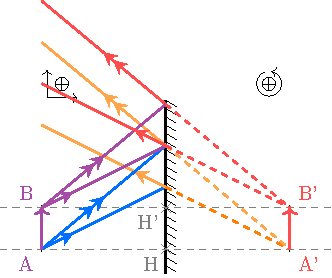
\includegraphics[width=.5\linewidth]{mir_plan-grand.pdf}
            \captionof{figure}{Image d'un objet étendu par un miroir plan.}
            \label{fig:mir_plan-grand}
        \end{center}
    \end{demo}
\end{tcbraster}

\section{Lentilles minces}
\subsection{Définition}

\begin{defi}[label=def:lents]{{lentilles, minces, convergentes et divergentes}}

    Une lentille est un composant optique \textbf{centré} constitué d'un milieu
    TLHI, délimité par deux dioptres de sommets $S_1$ et $S_2$. Elle est dite
    \textbf{mince} si son diamètre est très grand devant son épaisseur.

    \begin{defiside}

        Une lentille est \textbf{convergente} si son \textbf{point foyer objet}
        est \textbf{avant sa face d'entrée}.
        \begin{center}
            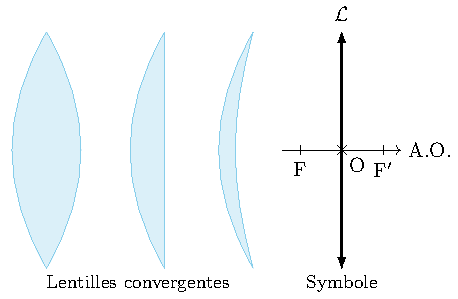
\includegraphics[height=3cm]{lent_conv-def.pdf}
            \captionof{figure}{Exemples de lentilles convergentes.}
            \label{fig:lent_conv-def}
        \end{center}

        \tcblower

        Une lentille est \textbf{divergente} si son \textbf{point foyer objet}
        est \textbf{après sa face de sortie}.
        \begin{center}
            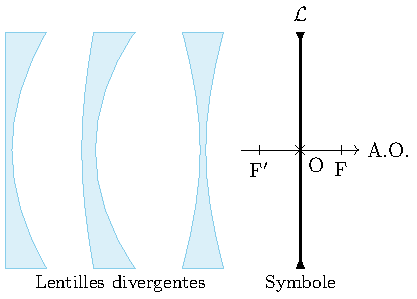
\includegraphics[height=3cm]{lent_div-def.pdf}
            \captionof{figure}{Exemples de lentilles convergentes.}
            \label{fig:lent_conv-def}
        \end{center}
    \end{defiside}
\end{defi}

    
\begin{ror}[label=impo:lent_gauss, hand]{stigmatisme et aplanétisme}

    D'une manière générale, les lentilles minces ne sont ni stigmatiques ni
    aplanétiques. Nous utiliserons donc toujours les lentilles minces dans
    les \textbf{conditions de Gauss} et les considérerons comme stigmatiques
    et aplanétiques.

\end{ror}

\subsection{Caractéristiques}

\begin{tcbraster}[raster columns=2, raster equal height=rows]
    \begin{defi}[label=def:co]{centre optique}

        On appelle \textbf{centre optique} d'une lentille et on le note $O$ le
        point à l'intersection de l'axe optique et de la lentille.

    \end{defi}
    \begin{prop}[label=prop:co]{centre optique et foyers}

        Tout rayon passant par le centre optique $O$ d'une lentille mince
        \textbf{n'est pas dévié}, et $F'$ est \textbf{symétrique} de $F$ par
        $O$.

    \end{prop}
    \begin{defi}[label=def:fv, raster multicolumn=2]{distance focale image
        et vergence}
        \begin{defiside}
            
            On appelle \textit{distance focale image} la distance
            \textbf{algébrique} $\OF$~; elle est positive pour une lentille
            convergent, négative pour une lentille divergente. \textbf{Elle se
            note usuellement $f'$}.

            \tcblower

            On appelle \textit{vergence} et on note $V$ la grandeur définie par
            \[ \boxed{V = \frac{1}{\OF}}\]

        \end{defiside}
        \tcbsubtitle[
        colback=green!50!black,
        colframe=green!50!black]{Unités}
        \begin{defiside}
            En tant que distance, $\OF$ (ou $f'$) s'exprime en mètres (m).
            \tcblower
            L'unité de la vergence est le \si{m^{-1}}, mais elle s'exprime
        usuellement en \textbf{dioptries} ($\delta$).
        \end{defiside}
    \end{defi}
\end{tcbraster}

\subsection{Constructions géométriques d'une lentille mince}
\subsubsection{Rappel}

\begin{rapp}[label=rapp:foy]{foyers d'une lentille}

    Par définition (voir chapitre 2), le \textbf{foyer objet} $F$ donne une
    \textbf{image à l'infini}, et ce \textbf{\underline{peu importe la nature de
    la lentille}}.\bigbreak

    De même, le \textbf{foyer image} $F'$ est le point \textbf{image} d'un
    \textbf{objet à l'infini}.

\end{rapp}
\begin{exem}[label=exem:lentfoy, sidebyside]{foyers des lentilles}
    \begin{center}
        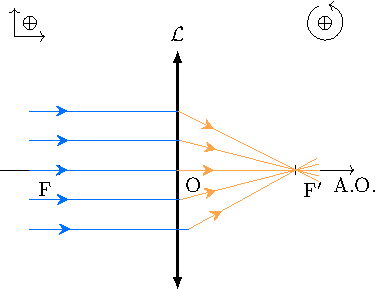
\includegraphics[width=\linewidth]{lent_conv-Fp}
        \captionof{figure}{Foyer image convergent}
        \label{fig:convfp}
    \end{center}
    \tcblower
    \begin{center}
        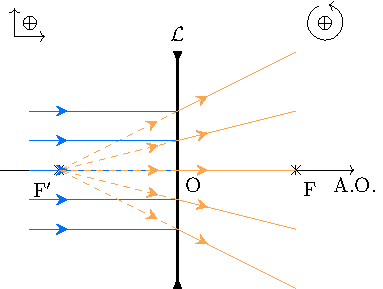
\includegraphics[width=\linewidth]{lent_div-Fp}
        \captionof{figure}{Foyer image divergent}
        \label{fig:divfp}
    \end{center}
\end{exem}

\subsubsection{Règles primaires}

\begin{tcbraster}[raster columns=2, raster equal height=rows]
    \begin{ror}[label=impo:lent_regles, hand]{règles primaires}
        Avec la propriété des foyers principaux, on a donc 3 points d'intérêts
        pour construire les rayons émergents d'une lentille mince~:
        \begin{enumerate}
            \item Tout rayon incident passant par $O$ n'est pas dévié~;
            \item Tout rayon incident parallèle à l'axe optique émerge en
                passant par $F'$.
            \item Tout rayon incident passant par $F$ émerge parallèle à l'axe
                optique~;
        \end{enumerate}
    \end{ror}
    \begin{exem}[label=exem:constru]{cas simple}
        \begin{center}
            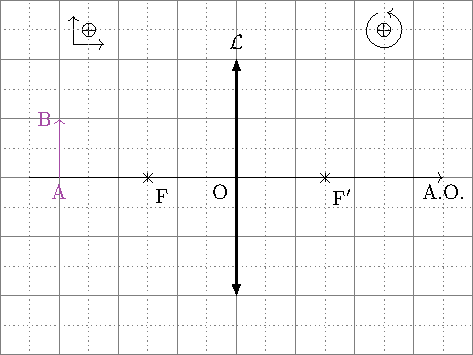
\includegraphics[width=\linewidth]{lent_conv-constru_simple-plain.pdf}
            \captionof{figure}{Utilisation des règles primaires}
            \label{fig:convconstrusimple}
        \end{center}
    \end{exem}
\end{tcbraster}
\begin{impo}[label=impo:cons_exem]{exemples de situations à compléter}
    \begin{minipage}{0.50\linewidth}
        \begin{center}
            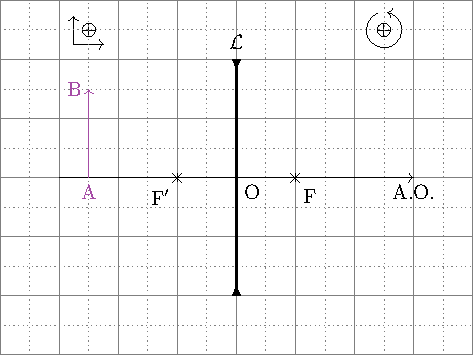
\includegraphics[width=\linewidth]{lent_div-constru_simple-plain.pdf}
            \captionof{figure}{Divergente simple}
            \label{fig:divconstrusimple}
        \end{center}
    \end{minipage}
    \hfill
    \begin{minipage}{0.50\linewidth}
        \begin{center}
            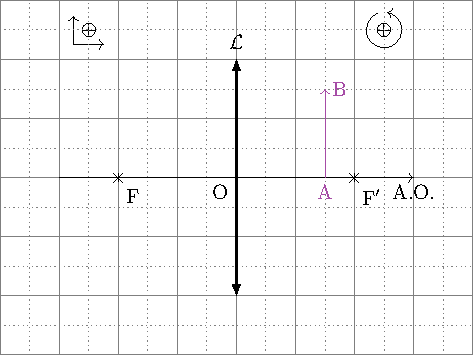
\includegraphics[width=\linewidth]{lent_conv-constru_after-plain.pdf}
            \captionof{figure}{Convergente après}
            \label{fig:convconstruafter}
        \end{center}
    \end{minipage}
    \begin{minipage}{0.50\linewidth}
        \begin{center}
            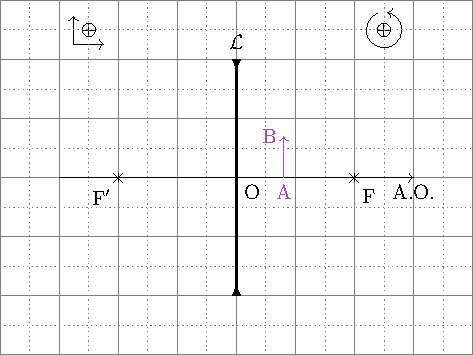
\includegraphics[width=\linewidth]{lent_div-constru_after_a-plain.pdf}
            \captionof{figure}{Divergente après}
            \label{fig:divconstruafter}
        \end{center}
    \end{minipage}
    \hfill
    \begin{minipage}{0.50\linewidth}
        \begin{center}
            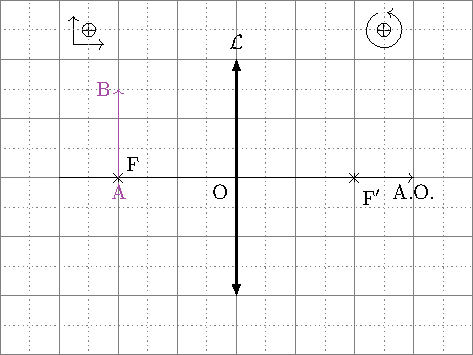
\includegraphics[width=\linewidth]{lent_conv-constru_F-plain.pdf}
            \captionof{figure}{Convergente $F$}
            \label{fig:convconstruF}
        \end{center}
    \end{minipage}
\end{impo}

\subsubsection{Règles secondaires}
\begin{tcbraster}[raster columns=2, raster equal height=rows]
    \begin{ror}[label=impo:lent_regles, hand]{règles secondaires}
        Avec la propriété des foyers secondaires, on a deux règles de
        construction supplémentaires~:
        \begin{enumerate}[start=4]

            \item Deux rayons incidents parallèles entre eux émergent en se
                croisant dans le plan focal image~;
            \item Deux rayons incidents se croisant dans le plan focal objet
                émergent parallèles entre eux.

        \end{enumerate}
    \end{ror}
    \begin{exem}[label=exem:constru]{cas simple}
        \begin{center}
            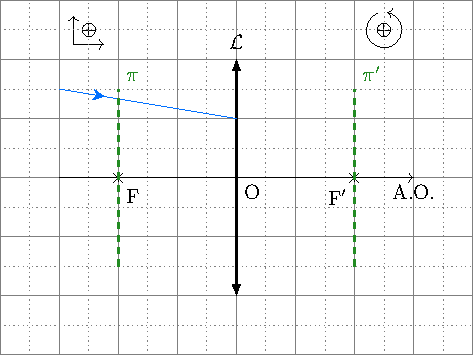
\includegraphics[width=\linewidth]{lent_conv-qqe-plain.pdf}
            \captionof{figure}{Utilisation des règles secondaires}
            \label{fig:convconstruqqe}
        \end{center}
    \end{exem}
\end{tcbraster}

\subsection{Corrigé des tracés}

\begin{exem}[label=exem, sidebyside]{Cas simple}
    \begin{center}
        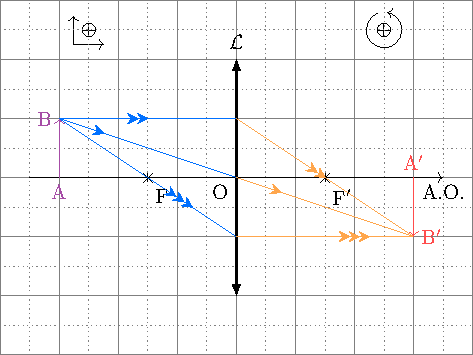
\includegraphics[width=\linewidth]{lent_conv-constru_simple.pdf}
        \captionof{figure}{Utilisation des règles primaires}
        \label{fig:corrconvconstrusimple}
    \end{center}
    \tcblower
    \begin{center}
        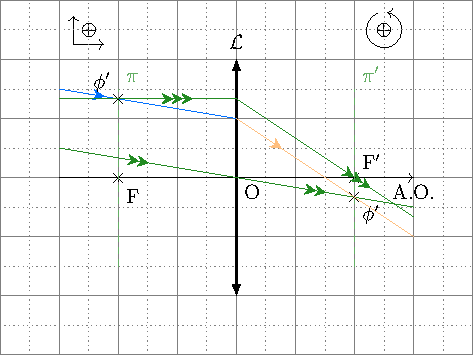
\includegraphics[width=\linewidth]{lent_conv-qqe.pdf}
        \captionof{figure}{Utilisation des règles secondaires}
        \label{fig:convconstruqqe}
    \end{center}
\end{exem}
\begin{impo}[label=impo:cons_exem]{exemples de situations à compléter}
    \begin{minipage}{0.50\linewidth}
        \begin{center}
            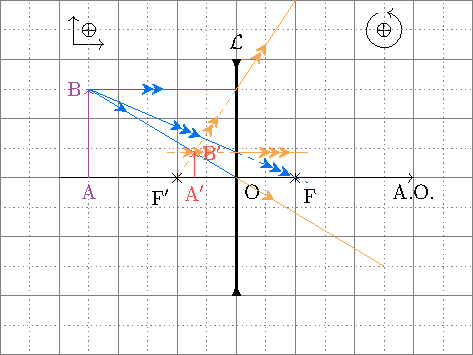
\includegraphics[width=\linewidth]{lent_div-constru_simple.pdf}
            \captionof{figure}{Divergente simple}
            \label{fig:corrdivconstrusimple}
        \end{center}
    \end{minipage}
    \hfill
    \begin{minipage}{0.50\linewidth}
        \begin{center}
            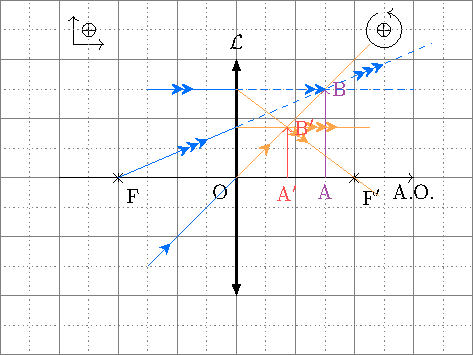
\includegraphics[width=\linewidth]{lent_conv-constru_after.pdf}
            \captionof{figure}{Convergente après}
            \label{fig:corrconvconstruafter}
        \end{center}
    \end{minipage}
    \begin{minipage}{0.50\linewidth}
        \begin{center}
            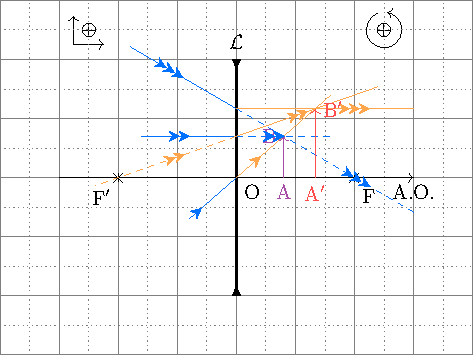
\includegraphics[width=\linewidth]{lent_div-constru_after_a.pdf}
            \captionof{figure}{Divergente après}
            \label{fig:corrdivconstruafter}
        \end{center}
    \end{minipage}
    \hfill
    \begin{minipage}{0.50\linewidth}
        \begin{center}
            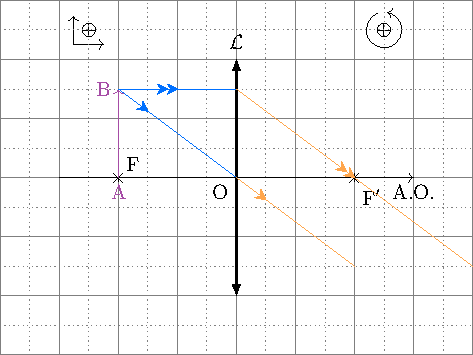
\includegraphics[width=\linewidth]{lent_conv-constru_F.pdf}
            \captionof{figure}{Convergente $F$}
            \label{fig:corrconvconstruF}
        \end{center}
    \end{minipage}
\end{impo}

\subsection{Relations de conjugaisons}

\begin{prop}[label=prop:conjdescartes, heart]{relations de conjugaison}
    Soit $\mathcal{L}$ une lentille de centre optique $O$ et de foyers $F$
    et $F'$, réalisant l'image $A'$ d'un objet $A$. On écrit
    \[ \boxed{A \opto{\Lc}{O} A'}\]
    et on a

    \begin{propside}

        \[\boxed{ \frac{1}{\OF} = \frac{1}{\OAp} - \frac{1}{\OA}}\]

        Relation de conjugaison de Descartes, avec origine au centre.

        \tcblower

        \begin{empheq}[box=\fbox]{align*}
            \OF\times\obar{OF}    & = \obar{F'A'}\obar{FA}\\
            \Leftrightarrow -f'^2 & = \obar{F'A'}\obar{FA}
        \end{empheq}
        Relation de conjugaison de Newton, avec origine aux foyers

    \end{propside}
\end{prop}

\subsection{Grandissement transversal}

\begin{coro}[label=coro:lent_grand, heart]{$\gamma$ lentille mince}
    À partir de la définition du grandissement transversal $\gamma =
    \frac{\ABp}{\ABb}$, on peut définir

    \begin{coroside}
        \[\boxed{\gamma = \frac{\ABp}{\ABb} = \frac{\OAp}{\OA}}\]
        \tcblower
        \[\boxed{\gamma = \frac{\obar{F'A'}}{\obar{F'O}} = 
        \frac{\obar{FO}}{\obar{FA}}}\]
    \end{coroside}
\end{coro}

\subsection{Complément~: démonstrations des relations}

\begin{demo}[label=demo:lent_rc, breakable]{relations de conjugaison et grandissement}
    \begin{demoside}
        Soit $\Lc$ telle que $AB \opto{\Lc}{O} A'B'$. On a la figure ci-contre.

        Pour trouver la relation de conjugaison, nous utilisons les triangles
        $OAB$ et $OA'B'$ pour lesquels nous utilisons le théorème de Thalès.
        Nous avons directement la formule du grandissement de Descartes~:

        \begin{equation*}
            \boxed{\frac{\obar{A' B'}}{\obar{AB}} =
            \frac{\obar{OA'}}{\obar{OA}} = \gamma}
        \end{equation*}

        \tcblower
        \begin{center}
            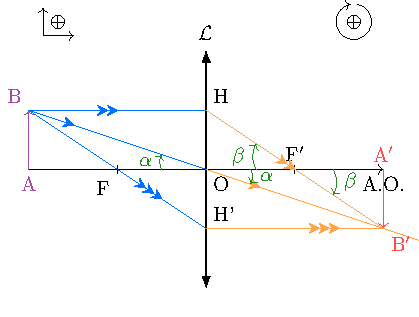
\includegraphics[width=\linewidth]{lent_conv-demo.pdf}
            \captionof{figure}{Schéma de notations}
            \label{fig:lent_rc}
        \end{center}
    \end{demoside}

    Nous définissons ensuite le point $H$ projeté orthogonal de $B$ sur
    la lentille, et le point $H'$ projeté orthogonal de $B'$ sur la lentille.

    \begin{demoside}
        En utilisant le théorème de Thalès dans les triangles $F'OH$ et
        $F'A'B'$ et en remarquant que $\obar{OH} = \ABb$, on a cette fois

        \begin{gather*}
            \frac{\obar{A'B'}}{\obar{OH}} = \frac{\ABp}{\ABb} =
            \frac{\obar{F'A'}}{\obar{F'O}}\\
            \Leftrightarrow \boxed{\gamma = - \frac{\obar{F'A'}}{\OF}}
        \end{gather*}
        \tcblower
        Et en utilisant les
        triangles $FAB$ et $FOH'$

        \begin{gather*}
            \frac{\obar{OH'}}{\obar{AB}} = \frac{\ABp}{\ABb} =
            \frac{\obar{FO}}{\obar{FA}}\\
            \Leftrightarrow \boxed{\gamma = - \frac{\obar{OF}}{\obar{FA}}}
        \end{gather*}
    \end{demoside}
    En les combinant on obtient élémentairement
    \begin{empheq}[box=\fbox]{align*}
        \OF\times\obar{OF}    & = \obar{F'A'}\obar{FA}\\
        \Leftrightarrow -f'^2 & = \obar{F'A'}\obar{FA}
    \end{empheq}

    En y injectant les décompositions
    \begin{equation*}
        \obar{F'A'} = \obar{F'O} + \obar{OA'}
        \quad\text{et}\quad
        \obar{FA} = \obar{FO} + \obar{OA}
    \end{equation*}
    et après développement, on obtient
    \begin{equation*}
        \OF\OAp - \OF\OA + \OA\OAp = 0
        \iff
        \boxed{\frac{1}{\obar{OF'}} =
        \frac{1}{\obar{OA'}} - \frac{1}{\obar{OA}}}
    \end{equation*}
    par division par $\OF\OA\OAp$.
\end{demo}

\section{Quelques applications}

\subsection{Condition de netteté}

Soit $AB \opto{\Lc}{O} A'B'$ avec $\Lc$ convergente projetant sur un écran. On
appelle $x$ la distance $ \left| \OA \right|$ et $D$ la distance fixe $AA'$.
Quelle est la contrainte sur le choix de lentille pour que $A'B'$ soit nette~?

\begin{tcbraster}[raster columns=2, raster equal height=rows]
    \begin{NCdefi}[]{Données}
        \begin{center}
            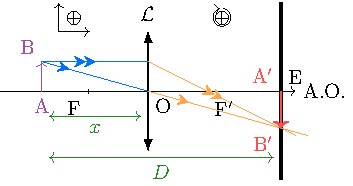
\includegraphics[width=\linewidth]{lent_conv-condition.pdf}
            \captionof{figure}{Schéma de situation}
            \label{fig:lent_condi}
        \end{center}
    \end{NCdefi}
    \begin{tcolorbox}[blankest, raster multicolumn=1]
        \begin{tcbraster}[raster columns=1]
            \begin{NCprop}[]{Résultat attendu}
                L'image est nette si la lentille forme l'image sur l'écran. Avec
                $D$ fixe, on cherche une équation avec $x$.
            \end{NCprop}
            \begin{NCrapp}[]{Outils}
                Relation de Descartes
                \[\boxed{ \frac{1}{\OF} = \frac{1}{\OAp} - \frac{1}{\OA}}\]
                et $\OA = -x$, $\OAp = D-x$.
            \end{NCrapp}
        \end{tcbraster}
    \end{tcolorbox}
\end{tcbraster}

\begin{NCexem}[sidebyside]{Application}
    Avec les notations de l'énoncé, la relation de Descartes devient
    \begin{align*}
        \frac{1}{f'} &= \frac{1}{D-x} - \frac{1}{-x}\\
        \Leftrightarrow \frac{1}{f'} &= \frac{x + D-x}{x(D-x)}\\
        \Leftrightarrow f' &= \frac{x(D-x)}{D}\\
        \Leftrightarrow 0 &= x^2 - xD + f'D 
    \end{align*}
    \tcblower
    Ce trinôme du second degré a pour discriminant $\Delta = D^2-4f'D =
    D(D-4f')$. $x$ étant une distance physique, on cherche $\Delta \geq 0$.
    \begin{itemize}
        \item $\Delta = 0$ si $D = 4f'$, et alors \[\boxed{x = \frac{D}{2}}\]
        \item $\Delta > 0$ si $D > 4f'$, et alors \[\boxed{x_\pm =
            \frac{D\pm\sqrt{D(D-4f')}}{2}}\]
    \end{itemize}
    Ainsi, la zone de netteté de l'image se situe entre $x_+$ et $x_-$, et a
    donc une largeur $d = x_+ - x_- = \sqrt{D(D-4f')}$.
\end{NCexem}

\subsection{Champ de vision à travers un miroir plan}
Une personne dont les yeux se situent à $h = \SI{1.70}{m}$ du sol observe une
mare gelée (équivalente à un miroir plan) de largeur $l = \SI{5.00}{m}$ et
située à $d = \SI{2.00}{m}$ d'elle.
\begin{enumerate}
    \item Peut-elle voir sa propre image~? Quelle est la nature de l'image~?
    \item Quelle est la hauteur maximale $H$ d'un arbre situé de l'autre côté de
        la mare (en bordure de mare) qu'elle peut voir par réflexion dans la
        mare~? On notera $D = l+d$.
\end{enumerate}

\subsubsection{Propre image}
\begin{tcbraster}[raster columns=2, raster equal height=rows]
    \begin{NCdefi}{Schéma}
        \begin{center}
            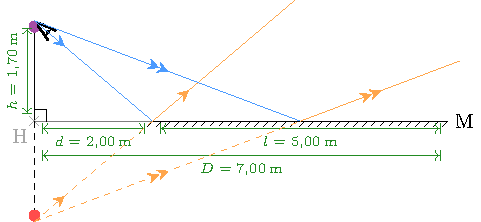
\includegraphics[width=\linewidth]{ch3-arbre-1}
        \end{center}
    \end{NCdefi}
    \begin{tcolorbox}[blankest, raster multicolumn=1, space to=\myspace]
        \begin{tcbraster}[raster columns=1]
            \begin{NCrapp}{Outil}
                Pour voir une image, il faut qu'un rayon partant de l'image
                puisse arriver jusqu'à l'œil de l'observataire. Étant donné
                qu'on travaille avec un miroir, l'image de l'observataire est
                son symétrique par le plan du miroir (même si le miroir ne
                s'étend pas jusque-là !).
            \end{NCrapp}
            \begin{NCexem}{Application}
                On voit vite qu'il n'est pas possible qu'un rayon issu de
                l'image (en rouge) atteigne l'œil (en violet). On comprend par
                le tracé des rayons réfléchis que seul l'autre côté du lac sera
                visible.
            \end{NCexem}
        \end{tcbraster}
    \end{tcolorbox}
\end{tcbraster}

\subsubsection{Image arbre}
\begin{tcbraster}[raster columns=2, raster equal height=rows]
    \begin{NCdefi}{Schéma}
        \begin{center}
            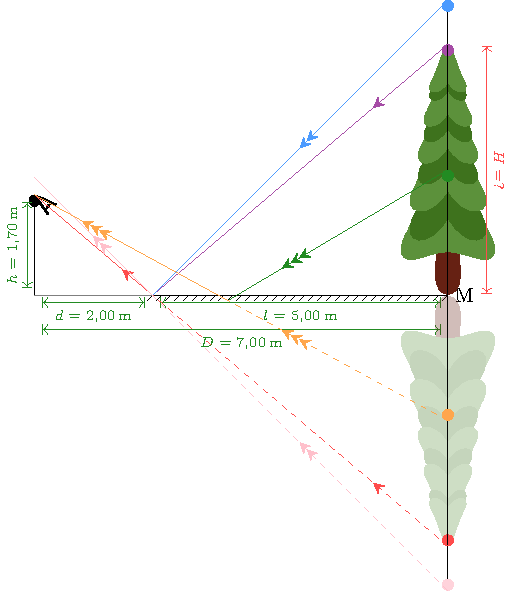
\includegraphics[width=\linewidth]{ch3-arbre-2}
        \end{center}
    \end{NCdefi}
    \begin{tcolorbox}[blankest, raster multicolumn=1, space to=\myspace]
        \begin{tcbraster}[raster columns=1]
            \begin{NCrapp}[add to natural height=\myspace]{Outil}
                Ici aussi, l'idée est de trouver l'image de l'arbre, et de voir
                la condition limite pour la taille visible.
            \end{NCrapp}
            \begin{NCexem}{Application}
                Un schéma avec l'image de l'arbre nous permet de voir que le
                point le plus haut qu'on peut voir par réflexion sur le lac est
                quand on regarde proche de nous : si on regarde plus loin, on
                voit en effet plus vers le bas de l'arbre (rayon vert incident,
                rayon orange émergent). Un arbre qui est trop grand ne sera pas
                visible en regardant ce point-là (rayon bleu incident, rose
                émergent). On s'intéresse donc à la construction géométrique
                formée par le rayon violet incident, rouge émergent, qui nous
                permet d'appliquer le théorème de Thalès : $\DS\frac{H}{l} =
                \frac{h}{d}$, soit
                \[\boxed{H = \frac{l\times h}{d}} \quad \text{avec} \quad
                    \left\{
                        \begin{array}{rcl}
                            l & = & \SI{5.00}{m}\\
                            h & = & \SI{1.70}{m}\\
                            d & = & \SI{2.00}{m}
                        \end{array}
                \right.\]
                D'où
                \[\boxed{H = \SI{4.25}{m}}\]
            \end{NCexem}
        \end{tcbraster}
    \end{tcolorbox}
\end{tcbraster}

%\theendnotes

\end{document}
